\section{Predicting Building Pressurization}

Building pressurization can be used as an effective ITS under the right circumstances.
However, determining this requires a measurement device to be installed, and moreover needs to record over some length of time to determine trends.
Thus, it would be desirable to use some more readily available metric, such as weather data, to predict building pressurization.\par

A variety of factors can contribute to determine overall building pressurization.
Some of these are artificially controlled and induced, such as the force convection by heating, ventilation, and air conditioning systems.
These are of course difficult to use to for prediction purposes, and can at some sites be the dominant means for controlling building pressurization, i.e. some buildings or rooms are forcefully pressurized to keep gases or contamination out.\par

Weather primarily contributes to building pressurization through two means.
The temperature difference between the interior of the building produces a density and subsequent pressure gradient on either side of the building wall - this is commonly called the \textit{stack effect}.
Wind striking the building also produces a pressure difference, the magnitude of which is largely dependent on wind speed.
However, if the building is pressurized or depressurized by this, is more complicated and generally depends on the wind direction and building characteristics; wind blowing on a leaky window causes a very different effect compared to a featureless wall.
Equations for predicting building pressurization as a function of weather is available in The American Society of Heating, Refrigerating and Air-Conditioning Engineers (ASHRAE) 2017 Handbook\cite{american_society_of_heating_2017_nodate} which is used as the primary source in this section.\par

These weather phenomena likewise can affect air exchange rates, and has been a significant focus in the VI modeling work by \citeauthor{shirazi_three-dimensional_2017}\cite{shirazi_three-dimensional_2017}.
As their work shows, predicting air exchange rate can be challenging, as accurate characterization often require detailed knowledge of the interior of a building, and will not be a focus in this work.\par

The study of the EPA duplex continuously monitored the indoor and outdoor temperature at the site and wind speed as well as its direction using an on-site weather station mounted on the roof of the building.
These data with the recorded indoor/outdoor pressure offers an opportunity how well building pressurization can be predicted using weather, which will be a focus on this section.
Ideally, the same would be done for the ASU house, but weather data at the site is not available to the author.\par

\subsection{Wind Effects}

To truly capture the impact that wind can have on a building and its pressurization, it is usually necessary to conduct wind tunnel tests of scale models of the building, or through detailed computational fluid dynamics (CFD) simulations.
This is especially true for buildings of even modest complex geometric shapes, where it is impossible to predict the wind pressure field without these tools.
However, it is possible to derive some simple equations to account for wind effects on simple rectangular block-type buildings.\par

Even with assumption, the inherent turbulent nature of wind means that is truly never at steady-state, and thus wind striking a wall generates a distribution of pressures across the surface, that can vary widely in a short period of time; resolving this with a high degree of accuracy requires a significant computational effort.
However, by considering the wind induced pressure field over some time-averaged period, it is possible to develop some simple equations for predicting wind induced pressurization for a rectangular building.
The drawback of this approach is that large pressure fluctuations will not be captured.\par

As the wind strikes the wall of a house, its velocity falls to zero, and the change in momentum is directly proportional to the change in pressure:
\begin{equation}\label{eq:wind_pressure_uncorrected}
  \Delta p_w = \frac{1}{2} \rho u_\mathrm{wind}^2
\end{equation}
where $\Delta p_w = p_\mathrm{wall} - p_\mathrm{wind}$ [\si{\pascal}] is the change in pressure at the building wall from the wind free-stream pressure;
$\rho_\mathrm{air}$ [\si{\kilo\gram\per\metre\cubed}] is the air density;
and $u_\mathrm{wind}$ [\si{\metre\per\second}] is the free-stream wind speed, here assumed to be the wind speed measured at some place where it is unaffected by terrain or buildings.\par

However, \eqref{eq:wind_pressure_uncorrected} neglects a variety of factors, such as terrain, vegetation, or other buildings.
It also neglects wind striking the wall at an angle.
These can be accounted for by introducing a drag or pressure coefficient $C_p$ into \eqref{eq:wind_pressure_uncorrected} giving \eqref{eq:wind_pressure}.
\begin{equation}\label{eq:wind_pressure}
  \Delta p_w = C_p \frac{1}{2} \rho u_\mathrm{wind}^2
\end{equation}
$C_p$ is a dimensionless number, varying between -1 and 1, and is a function of wind direction, the building itself, and immediate surrounding area.\par

Air density $\rho$ changes with temperature and barometric pressure, which can be accounted for via the ideal gas law.
\begin{equation}
  \rho = \frac{p_{bar}}{R_\mathrm{spec} T}
\end{equation}
here $p_{bar}$ [\si{\pascal}] is the barometric pressure;
$R_\mathrm{spec} = \SI{287.058}{\joule\per\kilogram\per\kelvin}$ is the specific gas constant for dry air;
and $T$ [\si{\kelvin}] is the ambient outside temperature.\par

To use \eqref{eq:wind_pressure} for predicting the EPA duplex pressurization, we need to choose some $C_p$ value; ideally, a CFD simulation of the structure would be used to determine $C_p$ as a function of the wind direction between 0 and 360 degrees.
There are some $C_p$ values available for some generic structures and cases in are available in the American Society of Civil Engineers book for building codes and standards\cite{simiu_design_nodate}.
However, none of these seem applicable to a duplex, nor seem to deal with the building located on the eastern side of the EPA duplex.
Instead we assume a generic $C_p = 0.35$, as values in this range are common.

Another factor to consider is that a building will be pressurized or depressurized by wind depending how leaky the wall it strikes is.
Generally, walls featuring doors, windows, or other opening will cause a depressurization, while a simple flat wall will cause a overpressurization effect\footnote{
It should be noted that this relationship is not always true, and will depend on the indoor/outdoor temperature difference, as well as the magnitude of the wind speed, as shown by \citeauthor{shirazi_three-dimensional_2017}\cite{shirazi_three-dimensional_2017}.
}.
By inspection of the EPA duplex, we see that all walls feature windows, but since we're only concerned with the pressurization of the heated side of the duplex (422, the right-hand side half in Figure \eqref{fig:indie_house}), we will assume that westerly wind overpressurizes the 422 side.\par

Wind direction was recorded in degrees relative to northerly wind at the EPA duplex, however, for simplicity we will divide these degrees up into eight cardinal directions (north, north-east, etc) and assign signs to indicate pressurization or depressurization respectively to each direction (see Table \ref{tbl:wind_direction}).\par

\begin{table}[htb!]
  \centering
  \begin{tabular}{c c c}
    \toprule
    Cardinal direction & Wind direction [\si{\degree}] & Pressurization sign \\
    \midrule
    N & $0 \pm 22.5$ & 1 \\
    NE & $45 \pm 22.5$ & 1 \\
    E & $90 \pm 22.5$ & 1 \\
    SE & $135 \pm 22.5$ & 1 \\
    S & $180 \pm 22.5$ & 1 \\
    SW & $225 \pm 22.5$ & 1 \\
    W & $270 \pm 22.5$ & -1 \\
    NW & $315 \pm 22.5$ & 1 \\
    \bottomrule
  \end{tabular}
  \caption{Division of wind direction into discrete cardinal directions with associated pressurization or depressurization of the EPA duplex.}
  \label{tbl:wind_direction}
\end{table}

\subsection{Temperature Effects}

The pressure of any fluid under the influence of gravity varies with elevation and the density of the fluid determines the magnitude of this pressure, which itself is function of the fluids absolute pressure and temperature.
If two columns of air are separated on either site of a wall at different temperatures, a pressure difference across the wall be induced, i.e. the \textit{stack effect}.\par

The pressure of air $p$ as a function of height above some reference plane at height $z_0$ is given by
\begin{equation}
  p = p_0 - \rho g z
\end{equation}
here $p_0$ [\si{\pascal}] is air pressure at reference plane $z_0$ [\si{\metre}];
$\rho$ [\si{\kilo\gram\per\metre}] is the density of air;
$g = \SI{9.82}{\metre\per\second\squared}$ is the acceleration due to gravity;
and $z$ [\si{\metre}] is the elevation above $z_0$.\par

Since we're concerned with predicting the stack effect for a relatively short building, we can neglect vertical air density gradients giving the horizontal pressure difference as:
\begin{equation}
  \Delta p_s = (\rho_{out} - \rho_{in}) g (z - z_0) = \rho_{out} \frac{T_{in} - T_{out}}{T_{in}} g (z - z_0)
\end{equation}
$\Delta p_s$ [\si{\pascal}] is the stack effect induced horizontal pressure difference;
$T$ [\si{\kelvin}] is the absolute temperature;
and the subscripts $in$ and $out$ are in reference to the indoor and outdoor values respectively.
Like in the wind effect section, air density is calculated as function of the barometric pressure and outside temperature.\par

As a reference height difference $\Delta z = z - z_0$, we use $\Delta z \approx \SI{-3}{\metre}$.
This based on the estimated height difference between the EPA duplex basement and some midpoint of the exterior of the building.
The recorded indoor/outdoor pressure difference at the EPA duplex is here defined as the pressure difference between wall-port 1 (WP-1), which was on the outside of the house, and the duplex basement.\par

\subsection{Air Exchange Rate}

It is possible to predict air exchange rate of a building using a similar approach to the one needed for pressure.
However, this approach requires detailed knowledge of the leakiness of a building and how different house compartments communicate, and thus is beyond the scope of this work.
Even if possible, air exchange rates were not continuously monitored at the EPA duplex, so evaluation of this approaches efficacy using the recorded weather data is difficult.
Predicting air exchange rate of a building by modelling is done in the VI modeling of \citeauthor{shirazi_three-dimensional_2017}\cite{shirazi_three-dimensional_2017}, which has had very positive results with their method so far.\par

\subsection{Predicting Pressurization At The EPA Duplex}

The indoor/outdoor pressure difference $p_{in}$ is assumed to be the sum of the stack effect ($\Delta p_s $) and wind contribution ($\Delta p_w$), here given simply by $p_s$ and $p_w$ respectively.
\begin{equation}
  p_{in} = p_s + p_w
\end{equation}
Figure \ref{fig:pressure_prediction} shows the recorded indoor/outdoor temperature difference and wind speed, how these two contribute individually to $p_{in}$, and how they contribute together to $p_{in}$ across the EPA duplex study period.\par

\begin{figure}[htb!]
  \centering
  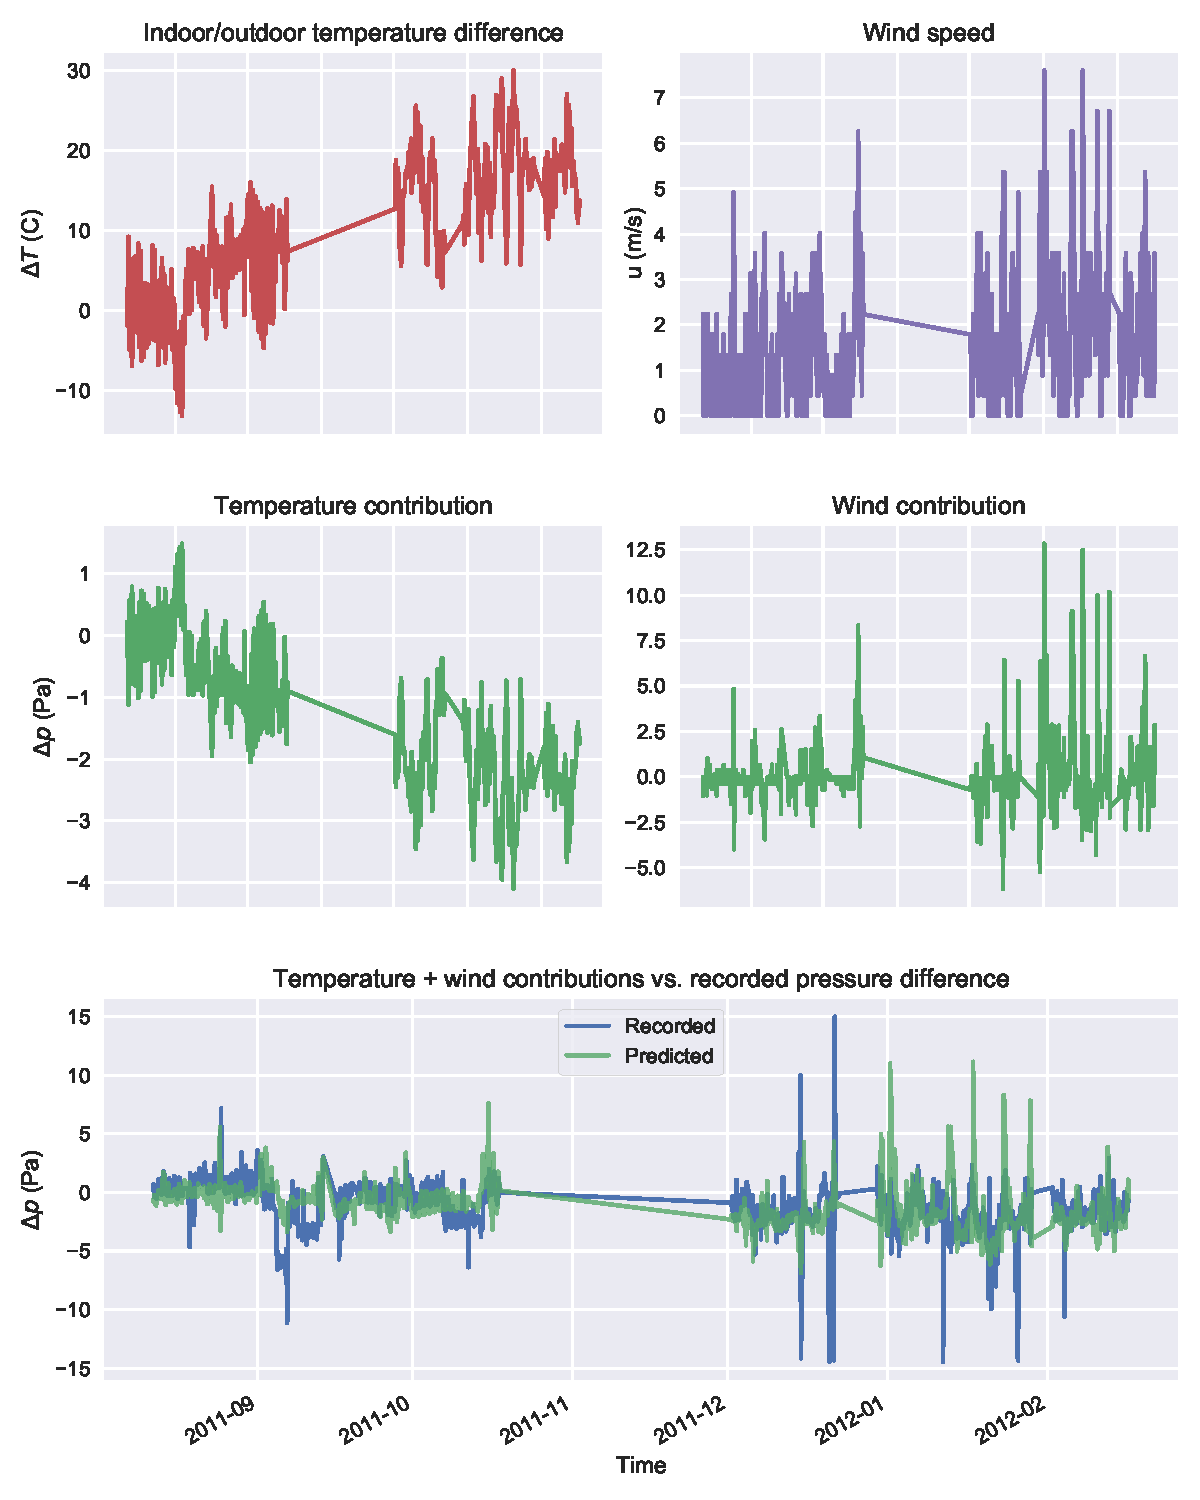
\includegraphics[width=\textwidth]{pressure_prediction.pdf}
  \caption{How indoor/outdoor temperature difference $\Delta T$ and wind contributes to building pressurization at the EPA duplex. The top left panel shows $\Delta T = T_{in} - T_{out}$, i.e. a positive value indicates that it is warmer indoors than outdoors. The top right shows the wind speed $u_\mathrm{wind}$. The middle panels shows the  contributions of $\Delta T$ and $u_\mathrm{wind}$ to $p_{in}$ respectively. The bottom panel shows the combined contribution of $\Delta T$ and $u_\mathrm{wind}$ to $p_{in}$, and compared to the recorded $p_{in}$ values. $p_{in} < 0$ indicates that the building is depressurized.}
  \label{fig:pressure_prediction}
\end{figure}

Figure \ref{fig:pressure_prediction} shows that with this relatively simple approach, the general trend of $p_{in}$ is captured.
Major errors seem to be mostly due to either a failure to capture large changes in $p_{in}$, or overpredict changes in $p_{in}$.
Both of these seem to stem from a relatively poor characterization of the wind influence, which strongly seems correlated with large changes in $p_{in}$ in general.\par

\begin{figure}[htb!]
  \centering
  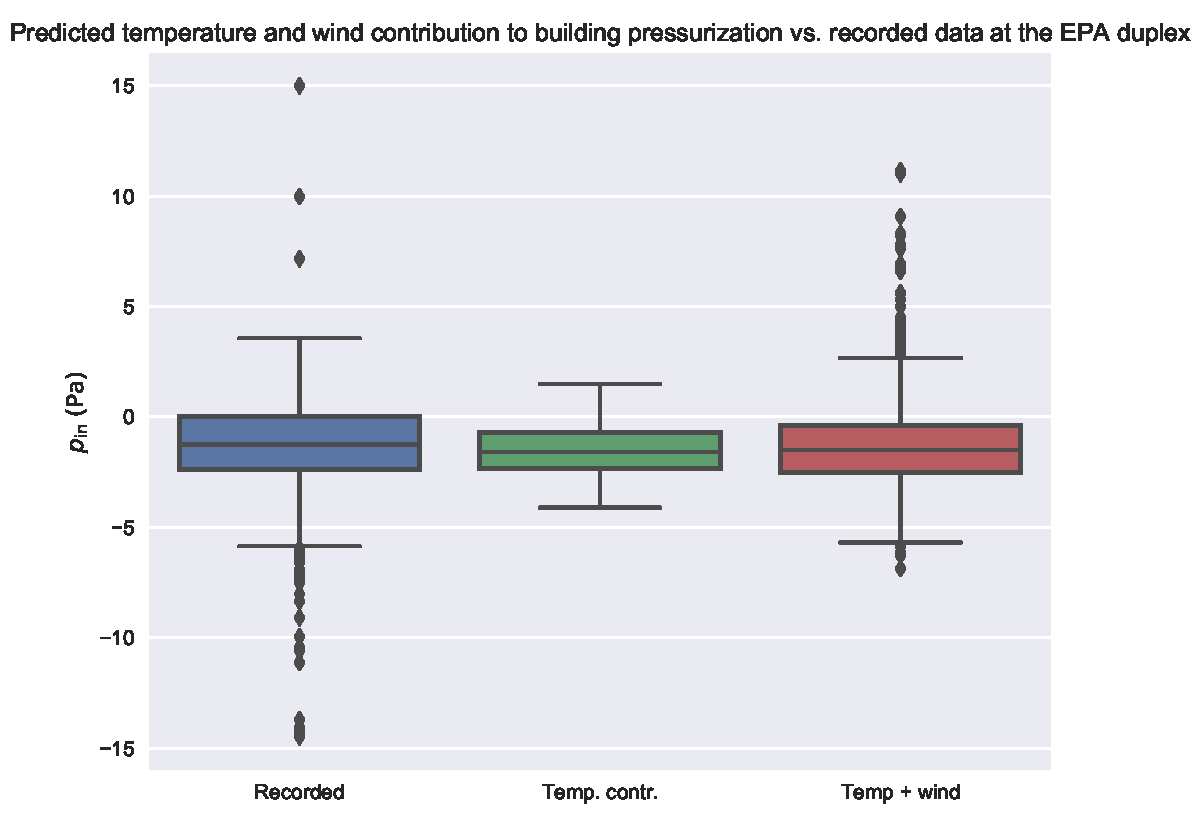
\includegraphics[width=0.75\textwidth]{pressure_prediction_boxplot.pdf}
  \caption{Boxplot comparing the predicted $p_{in}$ to the recorded values, and how the temperature and wind components contributes to the distribution of values.}
  \label{fig:pressure_prediction_boxplot}
\end{figure}

The differences and individual contributions of the temperature and wind effects can be further examined in Figure \ref{fig:pressure_prediction_boxplot} and Table \ref{tbl:pressure_prediction}. These show this approach reasonably predicts most of the $p_{in}$ distribution, specifically the mean pressurization and standard deviation are captured, but fails to capture, in particular, outliers where the building is significantly depressurized.
This is again due to poor account of the wind effect, and more advanced modeling of the influence of wind, such in the work by \citeauthor{shirazi_three-dimensional_2017}\cite{shirazi_three-dimensional_2017}, this is likely to be more well-captured.\par

\begin{table}[htb!]
  \centering
  \begin{tabular}{l c c c}
    \toprule
    & & \multicolumn{2}{c}{Predictions} \\ \cmidrule(r){3-4}
    & Data & $p_s$ & $p_s + p_w$ \\
    \midrule
    Mean & -1.33 & -1.50 & -1.31 \\
    Std. & 2.15 & 1.12 & 1.96 \\
    \bottomrule
  \end{tabular}
  \caption{Mean and standard deviation of recorded and predicted building pressurization. Here considering the temperature induced stack effect pressure difference $p_s$ alone, and the combined contribution of wind induced pressure difference $p_w$ and $p_s$.}
  \label{tbl:pressure_prediction}
\end{table}

Regardless, this approach shows that using temperature, wind, barometric pressure, and some simple assumptions about a building, it is possible to reasonably accurately characterize how building pressurization may change in the long-term and short-term.
This is in particular useful for planning when to conduct testing at sites that are more advection dominated, and one should here strive to collect samples when the building is continuously depressurized, i.e. when $\Delta T > \SI{5}{\degreeCelsius}$ and when there is little wind (to reduce uncertainty); this likely explains why it is often found that VI is most significant during colder months.
This gives credence to these weather factors as a reasonable ITS under certain circumstances.\par
